\section{Counting}

\subsection{Permutations}

Permutations are combinations where order matters. How permutations are calculated depends on whether repetitions are allowed or not. The number of permutations made from choosing $k$ from $n$ items when repetitions are allowed is $n^k$.

\begin{texample}
	Find the number of permutations of $ab$ when letters can be repeated. \\
	
	The permutations are: $aa, ab, ba, bb$. There is a total of $2^2=4$ permutations.
\end{texample}

When repetitions are not allowed, the number of permutations is just $n!$. Here is one way to understand where this formula came from: for the first item, there are $n$ choices to place and since no repetitions are allowed, there are $n-1$ choices left for the second item and so on.

\begin{texample}
	An Olympic final consists of two runners from each of four different countries. An ordered selection of three of the eight runners win the medals (gold, silver, and bronze). How many different possibilities are there if the medal winners are all from different countries? \\
	
	We are looking for an ordered selection of winners. There are $8$ choices for the gold medal winner. After the winner is chosen, since we want winners from different countries, there are $6$ options left for the solver medal winner. This leaves with $4$ options for the bronze medal winner. The total number of possible selections is therefore $8\times6\times4=192$.
\end{texample}

\begin{texample}
	Find the number of permutations of $abc$. \\
	
	The permutations are: $abc, acb, bac, bca, cab, cba$. There are total of $3(2!)=3!=6$ permutations. Three unique letters times the number of permutations of remaining letters. If there are 4 letters, the answer would be $4(3!)=24$.
\end{texample}

\begin{figure}[H]
	\centering
	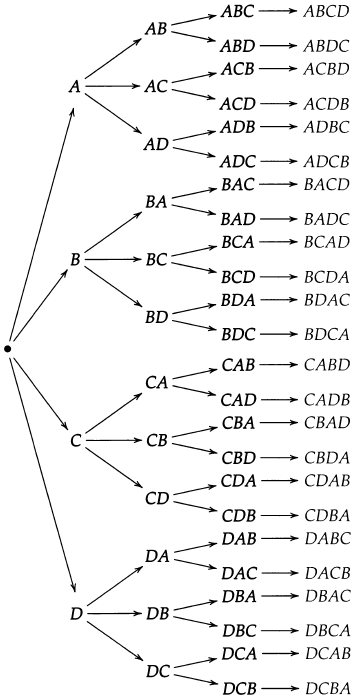
\includegraphics[width=60mm]{1.png}
	\caption{Permutations of $ABCD$ visualized}
\end{figure}

The above figure shows how to generate permutations of $ABCD$. We start with 4 choices for the first letter. Once we got the first letter, there are three choices remaining for the second letter and so on.

\begin{texample}
	Find the number of words created from rearranging letters $ALLELE$. \\
	
	There are two $E$s and three $L$s. Notice that there is no difference when you reorder these letters. Each word created from two $E$s and three $L$s corresponds to $2!3!$ permutations. \\
	
	The number of permutations is $6!$ which includes duplicates. To get the final answer, we divide it by $2!3!$ which gives $\frac{6!}{2!3!}=60$ total words.
\end{texample}

\begin{texample}
	Calculate the probability of obtaining exactly $3$ heads and tails for a total of 6 coin tosses. \\
	
	There are the total of $2^6=64$ possible outcomes. The number of times when the combination $HHHTTT$ occurs is $\frac{6!}{3!3!}=20$. Therefore the probability is $\frac{20}{64}=\frac{5}{16}$.
\end{texample}

To calculate the number of permutations made from choosing $k$ out of $n$ items with no repetition:

$$n(n-1)(n-2) \cdots (n-k+1)=\frac{n!}{(n-k)!}$$

It is usually denoted by ${}_n \mathrm{P}_k$.

\subsection{Combinations}

\begin{texample}
	How many ways to pick two out of $\{a, b, c, d\}$? \\
	
	Initially, there are four choices for the first letter of an ordered pair. After picking one, there are three choices left. There are $4(3)=12$ ordered pairs: $ab, ba, ac, ca, ad, da, bc, cb, bd, db, cd, dc$. However, we don't care about the order (ie. $ab$ and $ba$ is considered the same) so we divide by $2!$ which gives: $\frac{12}{2}=6$ combinations.
\end{texample}

To pick $k$ out of $n$ items, the total number of combinations is the number of ways to create ordered combinations (permutations) of size $k$ divided by the number of permutations of $k$ items in combinations. The calculation process is outlined below:

\begin{align*}
	\frac{n(n-1)(n-2) \cdots (n-k+1)}{k!} = \frac{\frac{n!}{(n-k)!}}{k!} = \frac{n!}{k!(n-k)!}
\end{align*}

We use $\binom{n}{k}$ to denote $\frac{n!}{k!(n-k)!}$. It is read as ``n choose k.'' This is a binomial coefficient. Another way to think about combinations is that it is the same as finding how many ways to rearrange $n$ cards where $k$ cards are coloured red and $n-k$ cards are coloured green. Also note that:

\begin{align*}
	\binom{n}{n-k} = \frac{n!}{(n-k)!(n-(n-k))!} = \frac{n!}{(n-k)!k!} = \binom{n}{k}
\end{align*}

$\binom{n}{k}$ is maximized when $k=n/2$.

\begin{texample}
	How many ways to deal $52$ cards to $4$ players? \\
	
	We count the number of ways to pick $13$ cards from the deck of $52$ cards. We then multiply it by the number of ways to pick another set of $13$ cards from the deck of $52-13=39$ cards. We multiply it again by the number of ways to pick another set of $13$ cards from the deck of $39-13=26$ cards. The remaining number of cards is $26-13=13$ which will be given to the last player.
	
	$$\binom{52}{13}\binom{39}{13}\binom{26}{13}\binom{13}{13}=\frac{52!}{(13!)^4}$$
\end{texample}

There is an interesting observation that can be used to calculate binomial coefficients. Suppose you toss a coin $n$ times and $k$ of $n$ tosses are heads. The number of possible ways to get $k$ heads out of $n$ tosses is given by $\binom{n}{k}$. To find this binomial coefficient, consider two cases: the first toss is H and the first toss is not H. When the first toss is H, the remaining tosses $n-1$ must have $k-1$ heads and the number of possible ways it can happen is $\binom{n-1}{k-1}$. When the first toss is not H,  the remaining tosses $n-1$ must have $k$ heads and the number of possible ways it can happen is $\binom{n-1}{k}$. The number of possible ways to get $k$ heads out of $n$ tosses is the number of possible ways to get H as the first toss plus the number of possible ways not to get H as the first toss:

$$\binom{n}{k} = \binom{n-1}{k-1} + \binom{n-1}{k}$$

This is called ``Pascal's rule.'' It can be used to construct Pascal's triangle.

\begin{center}
	\begin{tabular}{rccccccccc}
		&    &    &    &    &  1\\\noalign{\smallskip\smallskip}
		&    &    &    &  1 &    &  1\\\noalign{\smallskip\smallskip}
		&    &    &  1 &    &  2 &    &  1\\\noalign{\smallskip\smallskip}
		&    &  1 &    &  3 &    &  3 &    &  1\\\noalign{\smallskip\smallskip}
		&  1 &    &  4 &    &  6 &    &  4 &    &  1\\\noalign{\smallskip\smallskip}
	\end{tabular}
\end{center}

$\binom{n}{k}$ gives the value at $n$th row and $k$th column (both zero-indexed) of the triangle. For example, in the third row and second column, $\binom{2}{1}=2$. Notice that the total in each row is always $2^n$.

\subsection{Multinomial Coefficient}

The binomial coefficient formula $\binom{n}{k}$ can also be thought of as the number of ways to distribute $n$ items into two boxes in such way that one box has $k$ items and the another has $n-k$ items. Multinomial coefficient generalizes this fact to multiple boxes. \\

The formula for the multinomial coefficient can be derived from binomial coefficients. Suppose you have $r$ boxes where you want to distribute (distinct) $n$ items. You want each box to have $k_1, k_2, k_3, \dots, k_r$ items with $k_1+k_2+\cdots + k_r=n$. You first count the number of ways to distribute $k_1$ items in the first box with $n-k_1$ items remaining and this gives $\binom{n}{k_1}$. Then using the remaining $n-k_1$ items to count the number of ways to distribute $k_2$ items in the second box which gives $\binom{n-k_2}{k_2}$. There are $n-k_1-k_2$ items left and this will be used to calculate the number of ways to distribute $k_3$ items into the third box and so on. The number of ways to distribute $n$ items into $m$ boxes is therefore:

\begin{align*}
	\binom{n}{k_1}\binom{n-k_1}{k_2}\binom{n-k_1-k_2}{k_3}\ldots\binom{k_{r-1}+k_r}{k_{r-1}}\binom{k_r}{k_r}
\end{align*}

Simplifying this expression gives multinomial coefficient:

\begin{align*}
	\boxed{\binom{n}{k_1, k_2, k_3, \dots, k_r} = \frac{n!}{k_1! k_2! k_3! \cdots k_r!}}
\end{align*}

This can also be interpreted as the number of words if letters appear $k_1, k_2, k_3, \dots, k_r$ times. The fourth example can also be solved with $\binom{6}{1, 2, 3}$.

\begin{texample}
	How many ways to arrange the sequence of letters $ABRACADABRA$ in such way that there are no consecutive $A$s? \\
	
	The position of $A$s must be five numbers from $\{1, 2, 3, \dots, 11\}$ with no two consecutive numbers. Denote positions of each of the five $A$s by $i,j,k,l,m$ and $i, j-1, k-2, l-3, m-4$ should not contain repetitions. This means $i, j-1, k-2, l-3, m-4$ should take five numbers from $\{1, 2, 3, \dots, 7\}$. There are $\binom{7}{5}=21$ possible sets of locations for the $A$s. For each of them, there are $\binom{6}{4,4}=180$ arrangements for the remaining letters. The overall answer is $21(180)=3780$.
\end{texample}

\subsection{Stars and Bars}

A graphical aid involving stars and bars can solve a wide range of problems. Let's walk over the following examples.

\begin{texample}
	There are $5$ buckets of ice cream, each with different flavour. How many ways to make $3$ scoops, provided repetitions are allowed?
	
	It is easier to solve this problem by considering this related problem. We first line up $5$ stars like this:
	
	$$\star\quad \star\quad \star\quad \star\quad \star$$
	
	We then replace a star with $3$ bars:
	
	$$\star\quad \star\quad \star\quad |||\quad \star$$
	
	A star means ``skip'' and a bar means ``serve.'' In this example, the first three ice cream buckets are skipped and all three scoops are from the fourth ice cream bucket. We reduced the original problem is reduced to: ``how many ways to arrange $4$ stars and $3$ bars in $4+3=7$ places?'' This gives $\binom{7}{3}=35$ ways.
\end{texample}

Number of combinations made from choosing $k$ items from $n$ when duplicates are allowed is summarized by the below formula:

$$\binom{n+k-1}{k}$$

\begin{texample}
	How many different possible face value combinations created from rolling $3$ dice? \\
	
	This is similar to the ice cream problem we did earlier but with $6$ different ice cream choices. The answer is ${6+3-1 \choose 3}=56$.
\end{texample}

\begin{texample}
	How many solutions does the equation $a+b+c=12$ have, where $a,b,c$ are non-negative integers? \\
	
	We first line up $12$ stars like this:
	
	$$\star\quad \star\quad \star\quad \star\quad \star\quad \star\quad \star\quad \star\quad \star\quad \star\quad \star\quad \star$$
	
	We then insert $2$ bars between the stars, for example:
	
	$$\star\quad \star\quad \star\quad |\star\quad \star\quad \star\quad \star\quad |\star\quad \star\quad \star\quad \star\quad \star$$
	
	Here, it represents one solution: $3+4+5=12$. We reduced the original problem is reduced to: ``how many ways to arrange $12$ stars and $2$ bars in $12+2=14$ places?'' The answer is $\binom{14}{2}=91$ solutions.
\end{texample}
